\begin{task}{1, Approximating functions}
In this task we want to implement basic approximation algorithms using linear least squares and radial basis functions. We demonstrate some basic use cases on (A) a linear data set \verb|linear_function_data.txt| and (B) a non-linear data set \verb|nonlinear_function_data.txt|. Both data sets contain 1000 data points in $\mathbb{R}^2$.

\paragraph{Implementation}
The implementation is split into a python notebook \verb|task_1.ipynb| for conducting the experiments and \verb|utils.py| which contains all function implementations. As general note our own implementations can achieve similar results as the library implementation. We believe that our implementation is numerically unstable and hence have different hyper-parameters, since the library implementation uses a $LU$-decomposition. Here is a short overview on the functions provided by \verb|utils.py|:

\begin{center}
    \bgroup
    \def\arraystretch{1.5}
    \begin{tabular}{ |l|l| } 
    \hline
    Function & Description\\
    \hline
    \verb|load_dataset(...)| & Load dataset by line. Has an option for\\
    & sorting and choosing the string to splice by.\\
    \hline
    \verb|prepare_data(...)| & A helper function that splits data into $x,y$\\
    & and adjusts the shape.\\
    \hline
    \verb|expand_data(...)| & Turns $x\in\mathbb{R}$ into $x\in\mathbb{R}^n$\\
    & by applying a list of functions on $x$.\\
    \hline
    \verb|lstsq_direct(...)| & A helper function with direct implementation\\
    & of the closed-form solution for least squares.\\
    \hline
    \verb|linear_lstsq(...)| & A wrapper function that uses input data to\\
    & approximate a function using linear least squares.\\
    &Has an option to use and library implementation instead.\\
    \hline
    \verb|rbf(...)| & A helper function to calculate a Gaussian\\
    & radial basis function.\\
    \hline
    \verb|rbf_lstsq(...)| & Wrapper function that uses input data to\\
    & approximate a function using radial basis functions.\\
    & Has an option to use and library implementation instead.\\
    \hline
    \verb|plot_comparison(...)| & Plot 2 different functions for comparison.\\
    \hline
    \end{tabular}
    \egroup
\end{center}

\paragraph{Part 1: Approximate dataset (A) with a linear function.}
In this task we approximate a linear function on the dataset \verb|linear_function_data.txt| using linear least squares. After importing the dataset it was sorted in ascending order by its first feature. We will approximate a coefficient matrix $A$ from the data by a linear function with bias $b=0$:
\begin{align*}
    \hat{f}(x)=Ax+b
\end{align*}

In Figure \ref{fig:t1_1} we plotted the results. We can immediately observe that linear least squares can easily capture the function in the linear data. The blue crosses are the data points from \verb|linear_function_data.txt|. The approximated function is plotted in orange. Figure \ref{fig:t1_1}(a) shows the results of using our own implementation of the linear least squares. Note that our implementation does not use the parameter \verb|cond|, which cutoffs singular values smaller than \verb|cond| times the largest singular value of $A$. By default \verb|cond| is always set to $1.0$. Figure \ref{fig:t1_1}(b) shows the results after using the library implementation. Additionally we included one sample execution time. Our implementation was faster, since it has less features compared to the library function. In the following tasks we will use the library implementation, since we assume it is more numerically robust.\\

\begin{minipage}{\linewidth}%
The results for the coefficient matrix $A$ is as follows:
\begin{align*}
    A_{\text{direct}} = 0.75000024,\quad A_{\text{library}} = 0.75000024
\end{align*}

We used the following parameters:
\begin{center}
    \bgroup
    \def\arraystretch{1.5}
    \begin{tabular}{ |l|c|c|c| }
    \hline
    & \verb|bias|  & \verb|cond| & execution time\\
    \hline
    Figure \ref{fig:t1_1}(a) & False &  /  & 0.000165\\
    \hline
    Figure \ref{fig:t1_1}(b) & False & 1.0 & 0.042042\\
    \hline
    \end{tabular}
    \egroup
\end{center}
\end{minipage}

\begin{figure}[H]
\centering
\subfigure[Our implementation]{
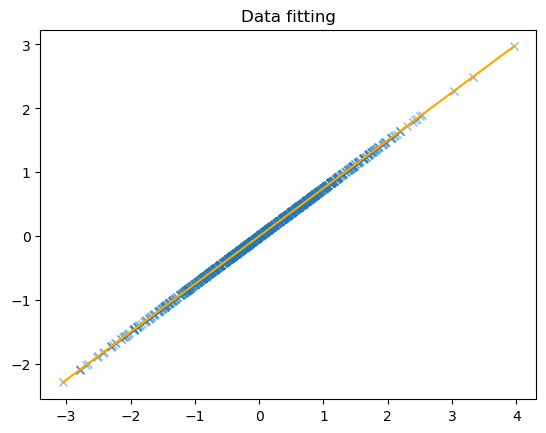
\includegraphics[width=0.45\textwidth]{images/t1-1.png}}
\subfigure[Library implementation]{
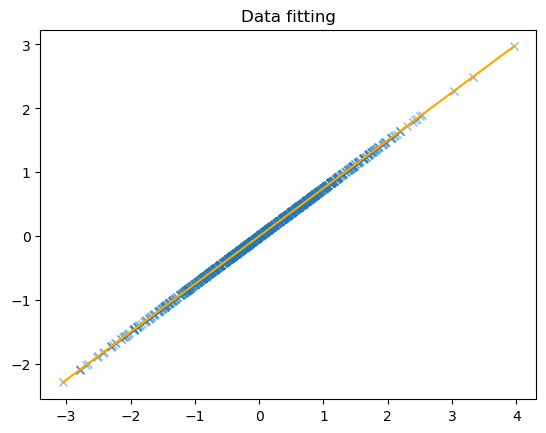
\includegraphics[width=0.45\textwidth]{images/t1-1lib.png}}
\caption{Plots of approximated functions on linear data}
\label{fig:t1_1}
\end{figure}

\paragraph{Part 1.1: Why is it not a good idea to use radial basis functions for dataset (A)?}
While linear least squares works perfectly fine on linear data, we might think of using a more powerful model, such as radial basis functions (RBF), to fit out data. This is generally a bad idea, if we can safely assume that our data is linear. There are many downsides to using a more powerful model like radial basis functions. The main downside in our case of Gaussian RBFs
%(Def. in \ref{})
is that we need to tune our hyper-parameters $L$ and $\epsilon$. Upon further analysis summarize what parameters are good

\begin{enumerate}
    \item We know that using a composition of non-linear transformations will likely result in a non-linear function if we use $L>2$. Therefore we can capture linearity only in the boundaries of our sample data.
    \item If we choose bad hyper-parameters then a bad i.e. non-linear fit will be visible within the range of the sample data. This can be see in figures \ref{fig:t1_1-rbf}(a)(b). But even good fit for $L>2$ will likely be non-linear. Hence it fits linear data incorrectly.
    \item The optimal choice would be $L=2$ and then trying to find a good $\epsilon$. But this $\epsilon$ can get quite large and overall it is a less efficient representation of linear data than linear least squares. A good fit using RBFs can be seen in figures \ref{fig:t1_1-rbf}(c)(d).
\end{enumerate}

In conclusion it is clear that theoretically RBFs are able to perfectly fit the data, but when used we need to tune hyper-parameters. Choosing bad hyper-parameters can be seen in figures \ref{fig:t1_1-rbf}(a)(b) and for $L>2$ the approximation is likely non-linear. Even if we can choose good hyper-parameters, $\epsilon$ can grow very large and it is overall a very inefficient representation of compared to linear least squares.\\


\begin{minipage}{\linewidth}%
The results for the coefficient matrix $C$ (of our implementation \ref{fig:t1_1-rbf}(a)(c) are as follows:
\begin{align*}
    C_{\text{Bad}}=(-1183008.2, -4276724.5, 25944456.4, ...),\quad C_{\text{Good}}=(-94.999,  95.341)
\end{align*}

We used the following parameters:
\begin{center}
    \bgroup
    \def\arraystretch{1.5}
    \begin{tabular}{ |l|c|c|c|c| }
    \hline
    & $L$ & $\epsilon$\\
    \hline
    Figure \ref{fig:t1_1-rbf}(a) & 100 & 1.2\\
    \hline
    Figure \ref{fig:t1_1-rbf}(b) & 100 & 1.2\\
    \hline
    Figure \ref{fig:t1_1-rbf}(c) & 2 & 0.1\\
    \hline
    Figure \ref{fig:t1_1-rbf}(d) & 2 & 1\\
    \hline
    \end{tabular}
    \egroup
\end{center}
\end{minipage}

\begin{figure}[H]
\centering
\subfigure[Our implementation]{
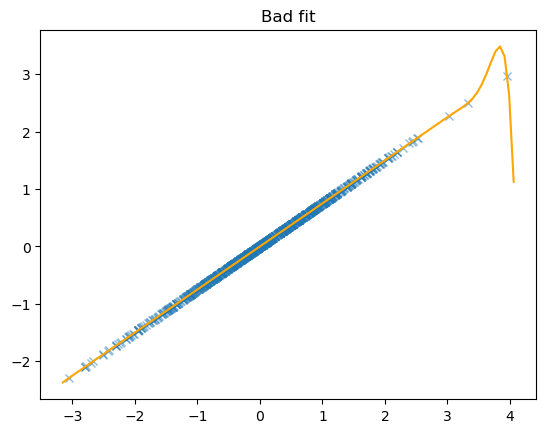
\includegraphics[width=0.45\textwidth]{images/t1-1a.png}}
\subfigure[Library implementation]{
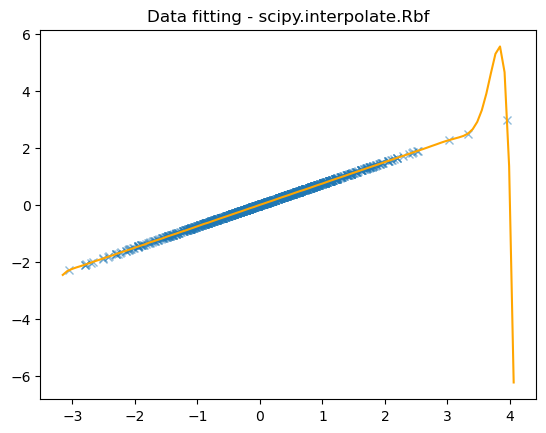
\includegraphics[width=0.45\textwidth]{images/t1-1b.png}}
\subfigure[Our implementation]{
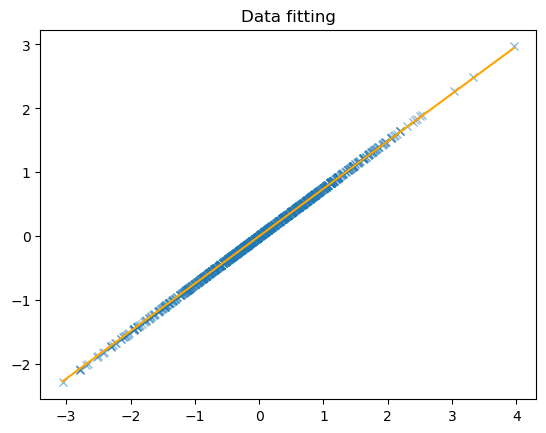
\includegraphics[width=0.45\textwidth]{images/t1-1c.png}}
\subfigure[Library implementation]{
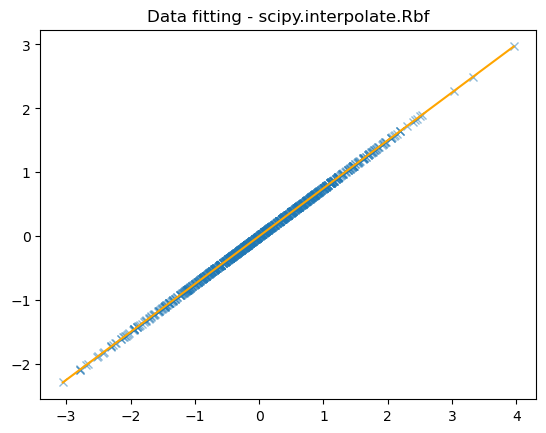
\includegraphics[width=0.45\textwidth]{images/t1-1d.png}}
\caption{Plots of approximated RBFs on linear data}
\label{fig:t1_1-rbf}
\end{figure}

\paragraph{Part 2: Approximate dataset (B) with a linear function.}
In this task we will try to approximate the non-linear dataset \verb|nonlinear_function_data.txt| with linear least squares. Again we have pairs of $x,y$ coordinates and sorted the data by its first feature $x$. We will approximate a coefficient matrix $A$ from the data, but this time we included the bias $b$ for the linear function $\hat{f}(x)=Ax+b$.

In Figure \ref{fig:t1_2} we have plotted the results only using our implementation of least squares. As expected the linear least squares is only able produce a linear function as approximation. Even though the resulting bias is very small we added it this time.

(As an additional remark we also extended the linear least squares to a Taylor series with polynomial of degree 13. In the python notebook \verb|task_1.ipynb| under task 1.2 it is interesting to see that we can achieve a nice fit using few polynomials. It is important to note that this model makes the assumption that the data has a certain polynomial behaviour.)

\begin{minipage}{\linewidth}%
The results for the coefficient matrix $A$ is as follows (note that bias $b$ is the second value in $A$):
\begin{align*}
    A = (0.02873498, 0.11114247)
\end{align*}

We used the following parameters:
\begin{center}
    \bgroup
    \def\arraystretch{1.5}
    \begin{tabular}{ |l|c|c| }
    \hline
    & \verb|bias|  & \verb|cond|\\
    \hline
    Figure \ref{fig:t1_2} & True & /\\
    \hline
    \end{tabular}
    \egroup
\end{center}
\end{minipage}

\begin{figure}[H]
\centering
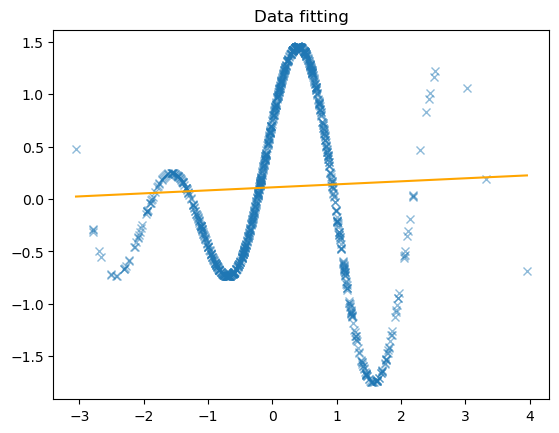
\includegraphics[width=0.45\textwidth]{images/t1-2.png}
\caption{Plots of approximated functions on linear data}
\label{fig:t1_2}
\end{figure}

\paragraph{Part 3: Approximate dataset (B) with a combination of radial functions.}
In this final part we are going to approximate the non-linear dataset using radial basis functions (RBF). Specifically here we are going to use a Gaussian RBF of the form:
\begin{align}
    \phi_l(x)=\text{exp}\left(\frac{||x_l -x_k||^2}{\epsilon^2}\right)
\end{align}

In figures \ref{fig:t1_3} we see an approximation using RBFs. Points were uniformly distributed and we receive a very smooth approximation of the dataset. On the left \ref{fig:t1_3}(a) is our own implementation, while the plot \ref{fig:t1_3}(b) uses the \verb|scipy| library implementation of RBFs. In our implementation it is possible to receive the coefficient matrix $C$.\\

\begin{minipage}{\linewidth}%
The results for the first 3 entries of the coefficient matrix $C$ are as follows:
\begin{align*}
    C= (483730.3, 2724108.7, -11428130.9, 5181098.3, 9651220.1)
\end{align*}

We used the following parameters:
\begin{center}
    \bgroup
    \def\arraystretch{1.5}
    \begin{tabular}{ |l|c|c|c| }
    \hline
    & $L$  & $\epsilon$\\
    \hline
    Figure \ref{fig:t1_3}(a) & 100 &  1.4\\
    \hline
    Figure \ref{fig:t1_3}(b) & 100 & 1.8\\
    \hline
    \end{tabular}
    \egroup
\end{center}
\end{minipage}

\begin{figure}[H]
\centering
\subfigure[Our implementation]{
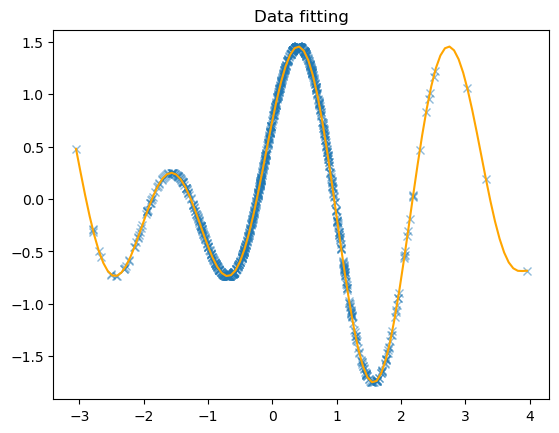
\includegraphics[width=0.45\textwidth]{images/t1-3.png}}
\subfigure[Library implementation]{
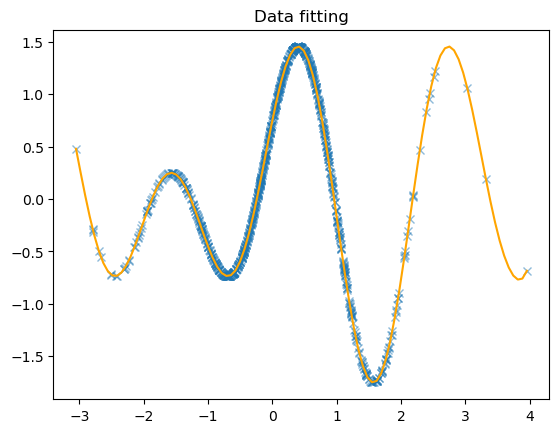
\includegraphics[width=0.45\textwidth]{images/t1-3a.png}}
\caption{Plots of approximated functions on non-linear data}
\label{fig:t1_3}
\end{figure}

\paragraph{Discuss how and why you chose the values of L and $\epsilon$ for the radial basis functions?}
As we have seen so far $L$ controls the amount of center points. This amount should be higher if the function is more complex. The non-linear dataset resembles a high-degree polynomial (Figure \ref{fig:t1_3}), hence choosing a decently large $L$ makes sense.

On the other hand as seen in part 1.1 choosing a smaller $L$ is appropriate when dealing with less data such as linear function data. Therefore we choose L=2 since we are dealing with a linear function. Overall the number of center points $L$ should be picked depending on the complexity of the functions curvature.\\

The hyper-parameter $\epsilon$ controls the bandwidth and inside the Gaussian RBF it acts as a scaling constant in the exponent. Intuitively it controls regularization strength and higher values force over-fitting. Generally choosing $\epsilon$ can vary by case, but a good rule of thumb could be to choose it as small as possible to prevent over-fitting.

Additionally using $\epsilon$ or $\epsilon^2$ for the Gaussian RBF makes no difference from a theoretical standpoint. But when taking tuning of hyper-parameters into consideration $\epsilon^2$ values increase quadratically and are better suited when trying to over-fit quickly. On the other hand a single $\epsilon$ is better for fine-tuning or working with data that is sensitive to regularization.
\end{task}